\documentclass[12pt]{beamer}

\mode<presentation> {
	\usetheme[blue,compress,numbers,nonav,nologo]{Trondheim}
	\usefonttheme[onlymath]{serif}
	\setbeamercovered{transparent}
}

%\usepackage{vub-beamer}
%\usepackage{vub_theme}

\setbeamertemplate{blocks}[rounded][shadow=true]

% The following makes latex use nicer postscript fonts.
\usepackage{times}

% zorg dat het ganse document in sans-serif is
\renewcommand{\familydefault}{\sfdefault}
\newcommand{\xmark}{\ding{55}}
\newcommand{\cmark}{\ding{51}}

% Math support
\usepackage{pifont}
\usepackage{amsmath}
\usepackage{amssymb}
\usepackage{amsfonts}
\usepackage{mathrsfs}
\setbeamertemplate{navigation symbols}{}%remove navigation symbols

%found. 
\usepackage{verbatim}

% put all math stuff in sans-serif
%\usepackage{sansmath}
%\sansmath

% Misc
%\usepackage[colorlinks,urlcolor=black,linkcolor=black,citecolor=black]{hyperref}
\usepackage{listings} % source listings
%\usepackage{multirow}
%\usepackage[times]{quotchap}
%\usepackage{setspace}

% Special words that latex has problem hyphenating.
\hyphenation{}

%\settaakheader
\title{GIT}
\subtitle{An Introduction}
\author{Roeland Matthijssens \& Bert Van Horenbeek}
\institute[] {Osudio}
\date[] {1 February 2016}
\subject{Beamer}

\usepackage{graphicx}
\usepackage{latexsym}
\usepackage{indentfirst}
\usepackage{xcolor}
\usepackage{listings}
\usepackage{tikz}
%\usepackage{amssymb}

\newcommand{\N}{\mathbb{N}}
\newcommand{\Z}{\mathbb{Z}}
\newcommand{\Q}{\mathbb{Q}}
\newcommand{\R}{\mathbb{R}}
\newcommand{\C}{\mathbb{C}}
\newcommand{\A}{\mathbb{A}}
\newcommand{\K}{\mathbb{K}}
\renewcommand{\H}{\mathbb{H}}
\renewcommand{\O}{\mathbb{O}}
\newcommand{\F}{\mathbb{F}}
\newcommand{\ltwee}{\mathnormal{l} ^2}

\newcommand{\dr}{\triangle}
\newcommand{\ring}{\C [\dr]}

\newcommand{\vect}{\mathrm{vect}}
\newcommand{\proj}{\mathrm{proj}}
\newcommand{\im}{\mathrm{Im}}
\newcommand{\ch}{\mathrm{char}}
\newcommand{\sig}{\mathrm{sig}}
\newcommand{\rang}{\mathrm{rang}}
\newcommand{\card}{\mathrm{card}}
\newcommand{\supR}{\mathrm{supR}}
\newcommand{\ann}{\mathrm{Ann}}

\definecolor{blurred}{rgb}{0.36,0.40,0.72}
\definecolor{dgreen}{rgb}{0.,0.6,0.}
\setbeamertemplate{background}{}
\begin{document}
	\begin{frame}
 \titlepage
\end{frame}

\section{Comparison}
	\begin{frame}
\frametitle{Core Ideas}
	\begin{block}{}
	\begin{itemize}
		\item Decentralised
		\item Fast
		\item Small
		\item Offline/Local version control
	\end{itemize}
	\end{block}
\end{frame}

	\subsection{Versioning Model}
	\begin{frame}
	\frametitle{Centralized}
	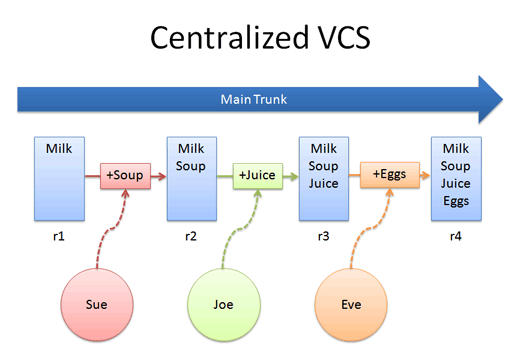
\includegraphics[width=\textwidth]{./images/centralized.png}
\end{frame}
\note[itemize]{
	\item linear versioning
	\item update before commit
	\item merge conflicts
	\item merging + branching is expensive
}
\begin{frame}
	\frametitle{Decentralized}
	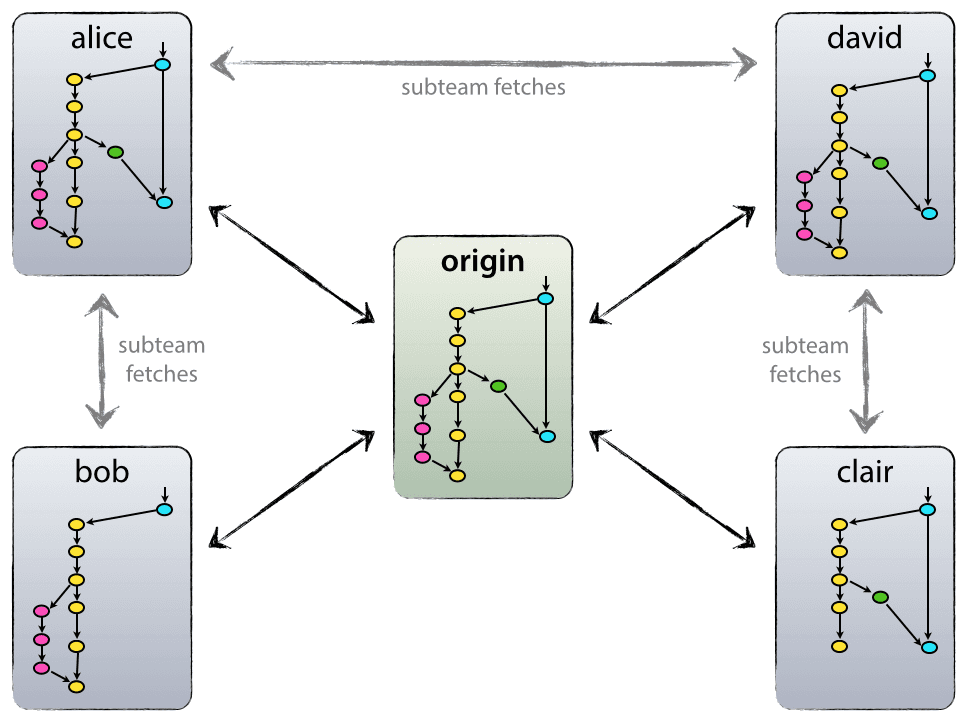
\includegraphics[width=\textwidth]{./images/decentralized.png}
\end{frame}
\note[itemize]{
	\item no notion of "latest" version
}


	\subsection{Smaller}
	\begin{frame}
\frametitle{Smaller}
\begin{block}{Some stats}
		Mozilla firefox project \newline
		10 year project, 240.000 commits \newline
		converted from svn to git \newline \newline
		\begin{tabular}{l | l | l}
			 & svn & git \\
			\hline
			size on disk & $\sim$3GB & 420MB \\
			size on server & $\sim$12GB & 420MB \\
			\#meta data files & 240.000 (1/commit) & 2 \\
			dupplication & per branch/tag & none \\
		\end{tabular}
	\end{block}
\end{frame}

\begin{frame}
	\begin{block}{Storage Model}
		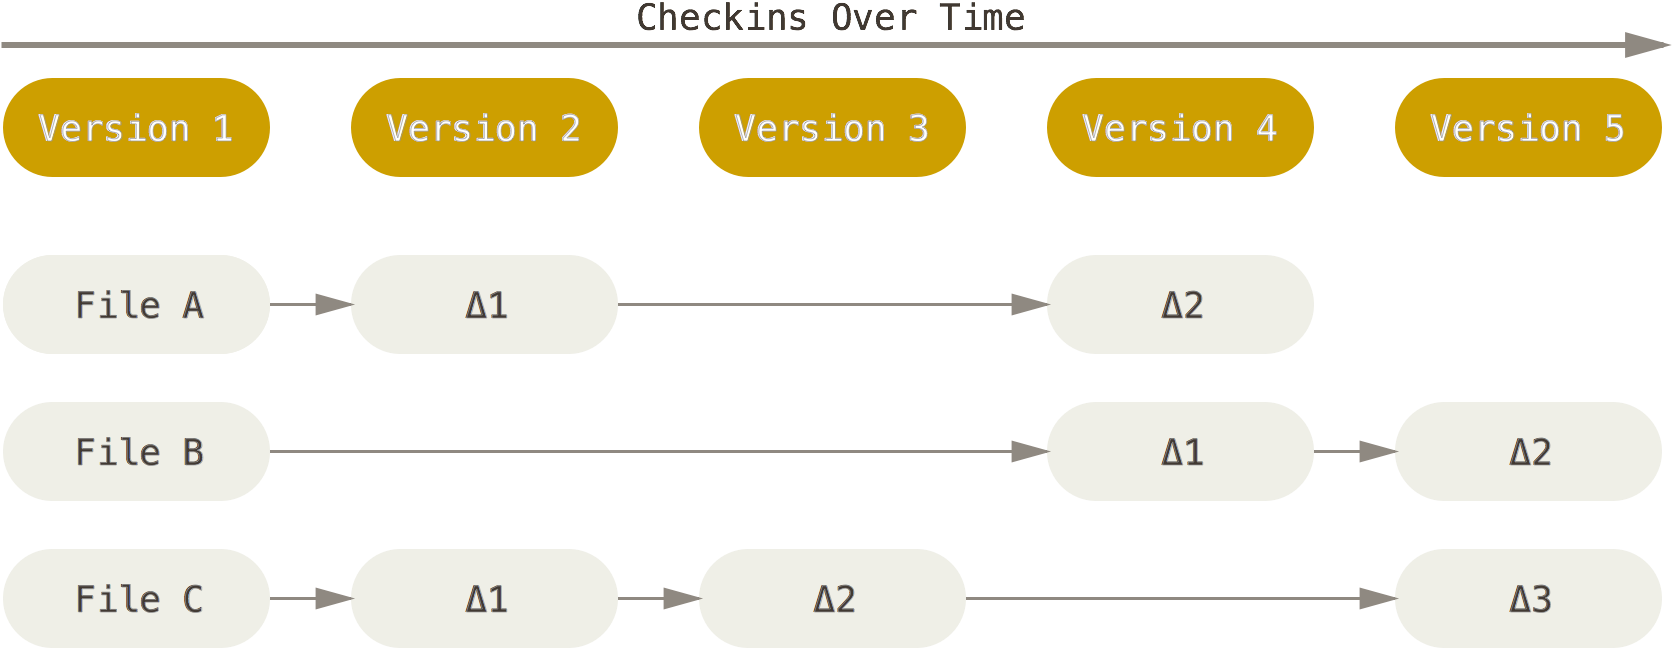
\includegraphics[width=\textwidth]{./images/deltaStorage.png}
	\end{block}
\end{frame}

	\subsection{Faster}
	\begin{frame}
	\begin{block}{Local repository}
		Entire history is stored locally. So no network latency
		\begin{itemize}
			\item no need to request old revision
			\item fast diffs
			\item fast commits
			\item fast revert
		\end{itemize}
	\end{block}
	\begin{block}{clone and pull?}
		\begin{itemize}
			\item Total repo size is small
			\item so clone is fast
			\item pull only retrieves deltas which are small
		\end{itemize}
	\end{block}
\end{frame}

	\subsection{Main Benefit}
	\begin{frame}
	\frametitle{Main Benefit}
	\begin{block}{Offline Versioning}
		Without network access we can still make use of our VCS
		\begin{itemize}
			\item Commit
			\item Revert
			\item Create branches
		\end{itemize}
	\end{block}
	\begin{block}{Local Versioning}
		\begin{itemize}
			\item Local sandboxing
			\item Breaking the repository only affect you
		\end{itemize}
	\end{block}
\end{frame}

\section{Basic Functionality}
\begin{frame}
	\frametitle{Summary}
	\begin{block}{}
		\begin{center}
			\begin{small}
				\begin{tabular}{|lcl|}
					\hline
					SVN & $\rightarrow$ & git \\
					\hline
					checkout & $\rightarrow$ & clone \\
					update & $\rightarrow$ & pull \\
					commit & $\rightarrow$ & commit + push \\
					log & $\rightarrow$ & log \\
					merge & $\rightarrow$ & merge/rebase \\
					copy & $\rightarrow$ & branch/tag \\
					diff & $\rightarrow$ & diff \\
					blame & $\rightarrow$ & blame \\
					\hline
				\end{tabular}
			\end{small}
		\end{center}
	\end{block}
\end{frame}

\begin{frame}
	\begin{block}{clone(svn=checkout)}
		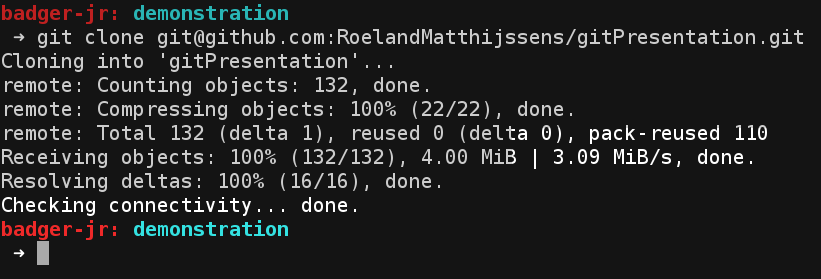
\includegraphics[width=\textwidth]{./images/clone.png}
	\end{block}
\end{frame}

\begin{frame}
	\begin{block}{pull(svn = update)}
		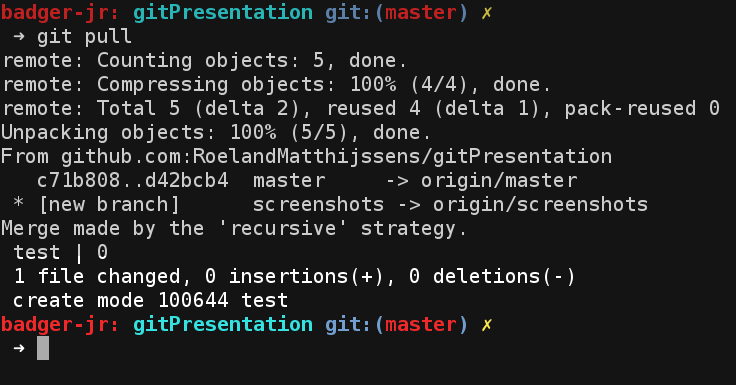
\includegraphics[width=\textwidth]{./images/pull.png}
	\end{block}
\end{frame}

\begin{frame}
	\begin{block}{commit (svn = NA)}
		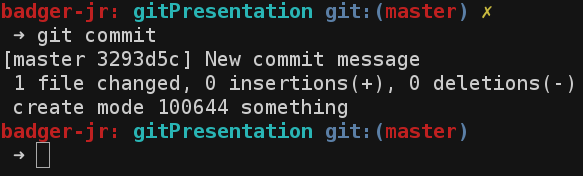
\includegraphics[width=\textwidth]{./images/commit.png}
		\newline
		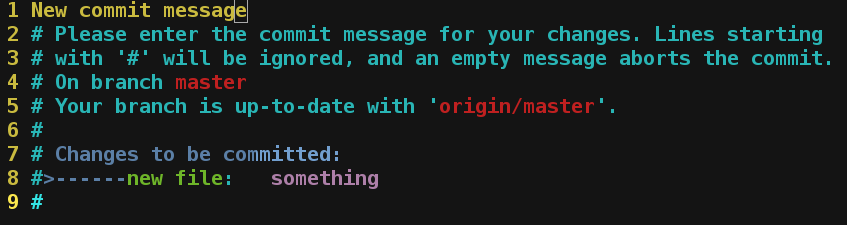
\includegraphics[width=\textwidth]{./images/commitMessage.png}
	\end{block}
\end{frame}

\begin{frame}
	\begin{block}{push (svn = commit)}
		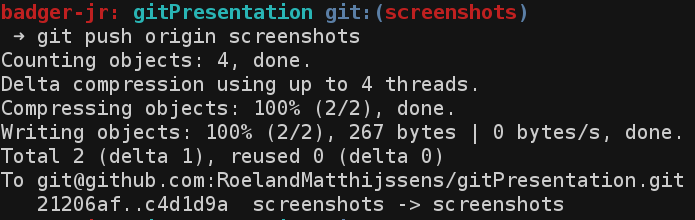
\includegraphics[width=\textwidth]{./images/push.png}
	\end{block}
\end{frame}

\begin{frame}
	\begin{block}{log}
		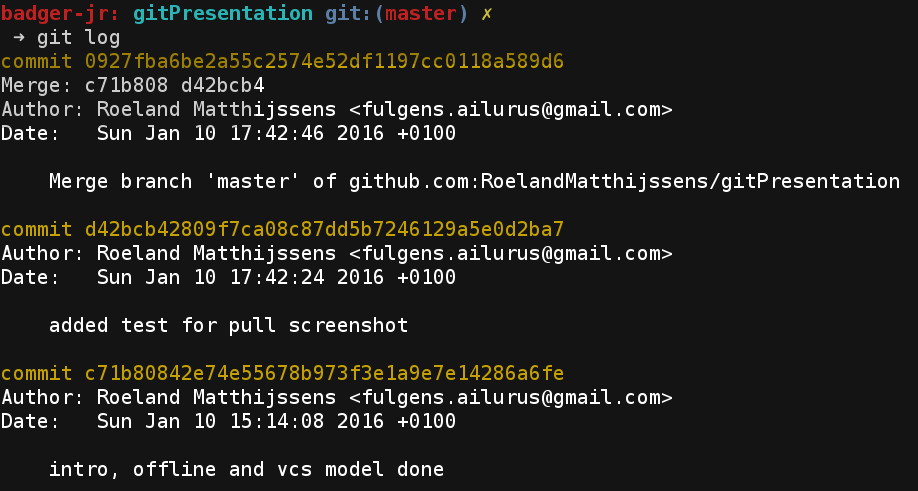
\includegraphics[width=\textwidth]{./images/log.png}
	\end{block}
\end{frame}

\begin{frame}
	\begin{block}{merge}
		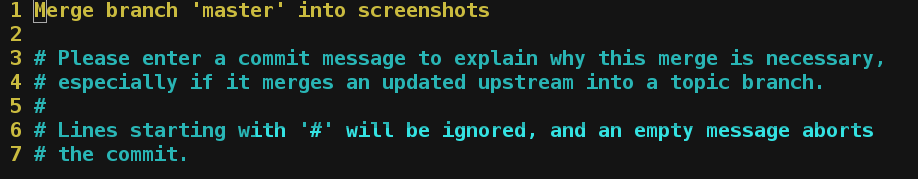
\includegraphics[width=\textwidth]{./images/mergeMessage.png}
		\newline
		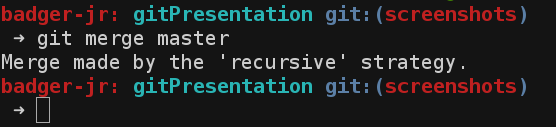
\includegraphics[width=\textwidth]{./images/merge.png}
	\end{block}
\end{frame}

\begin{frame}
	\begin{block}{branch(svn = copy)}
		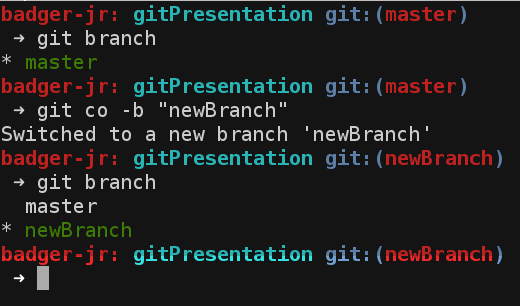
\includegraphics[width=\textwidth]{./images/branch.png}
	\end{block}
\end{frame}
\begin{frame}
	\begin{block}{checkout(svn = switch)}
		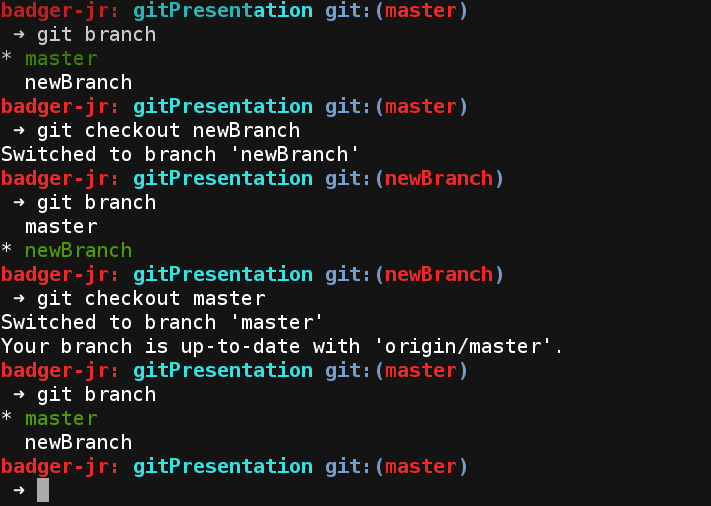
\includegraphics[width=\textwidth]{./images/checkout.png}
	\end{block}
\end{frame}
\begin{frame}
	\begin{block}{tag(svn = copy)}
		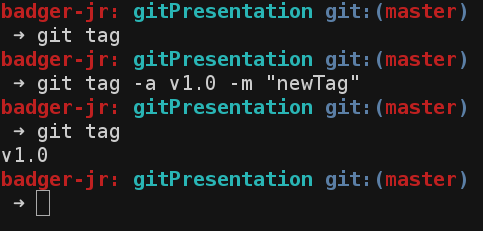
\includegraphics[width=\textwidth]{./images/tag.png}
	\end{block}
\end{frame}

\begin{frame}
	\begin{block}{diff}
		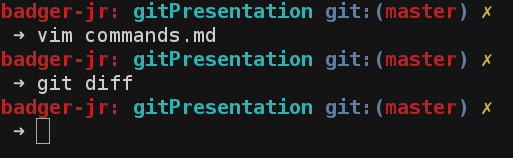
\includegraphics[width=\textwidth]{./images/diff.png}
		\newline
		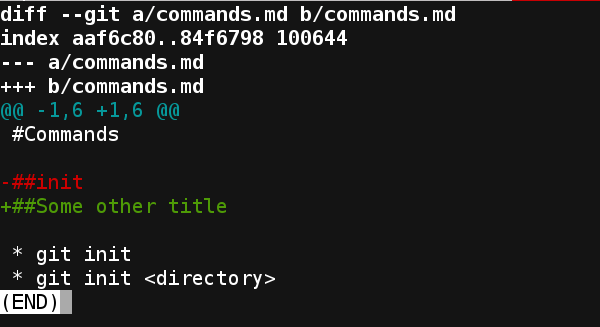
\includegraphics[width=\textwidth]{./images/diffMessage.png}
	\end{block}
\end{frame}

\begin{frame}
	\begin{block}{blame}
		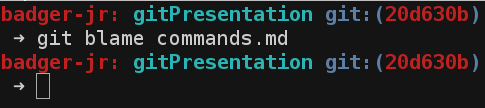
\includegraphics[width=\textwidth]{./images/blame.png}
		\newline
		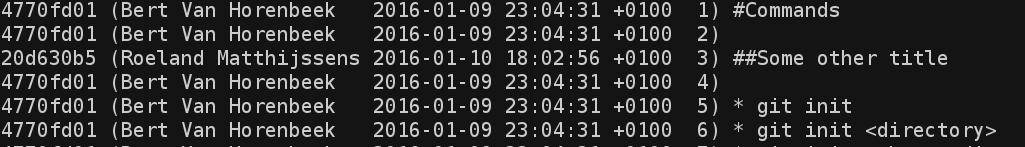
\includegraphics[width=\textwidth]{./images/blameMessage.png}
	\end{block}
\end{frame}

\begin{frame}
	\begin{block}{reset}
		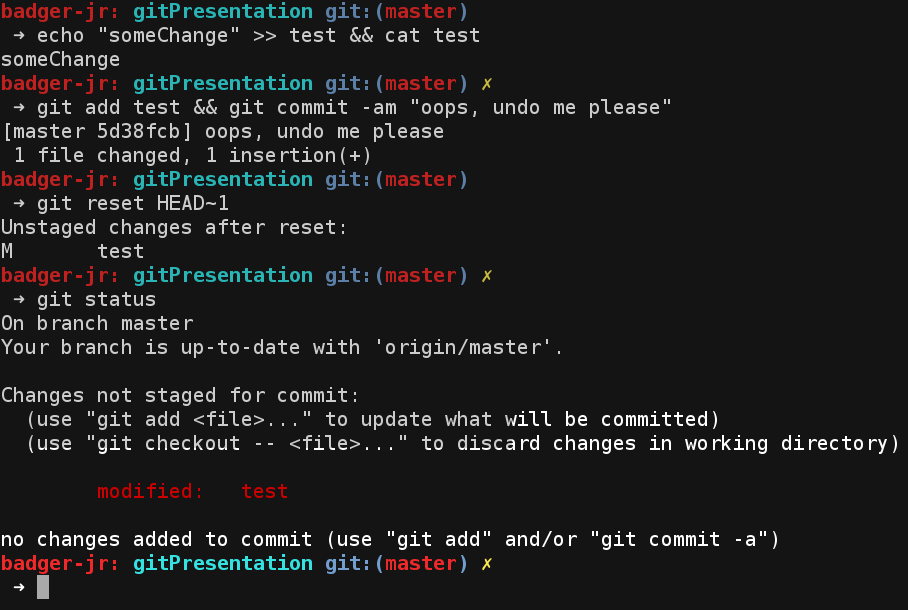
\includegraphics[width=\textwidth]{./images/reset.png}
	\end{block}
\end{frame}
\begin{frame}
	\begin{block}{reset --hard}
		svn equivalent = svn checkout -r $<revision>$ url://path/to/repo
		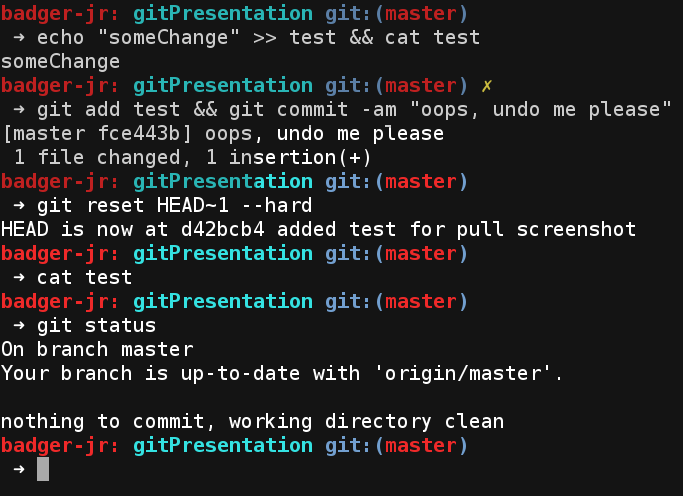
\includegraphics[width=\textwidth]{./images/resetHard.png}
	\end{block}
\end{frame}

\section{Tools}
\subsection{overview}
\begin{frame}
\frametitle{GUI tools}
	\begin{block}{}
		\begin{itemize}
			\item intellij/eclipse
			\item tortoise
			\item git lab
		\end{itemize}
	\end{block}
\end{frame}


\end{document}
